% This example is meant to be compiled with lualatex or xelatex
% The theme itself also supports pdflatex
\PassOptionsToPackage{unicode}{hyperref}
\documentclass[aspectratio=1610, 9pt]{beamer}

% Load packages you need here
\usepackage{polyglossia}
\setmainlanguage{german}

\usepackage{csquotes}
    

\usepackage{amsmath}
\usepackage{amssymb}
\usepackage{mathtools}

\usepackage{hyperref}
\usepackage{bookmark}

% load the theme after all packages

\usetheme[
  showtotalframes, % show total number of frames in the footline
]{tudo}

% Put settings here, like
\unimathsetup{
  math-style=ISO,
  bold-style=ISO,
  nabla=upright,
  partial=upright,
  mathrm=sym,
}

\title{PROPOSAL-Simulationsstudien zur Myographie in stillgelegten Bergbaustollen}
\author[M.~Schönfeld]{Martin Schönfeld}
\date{18. März 2022}
\institute[E5b]{E5b Astroteilchenphysik \\  Fakultät Physik - TU Dortmund}
\titlegraphic{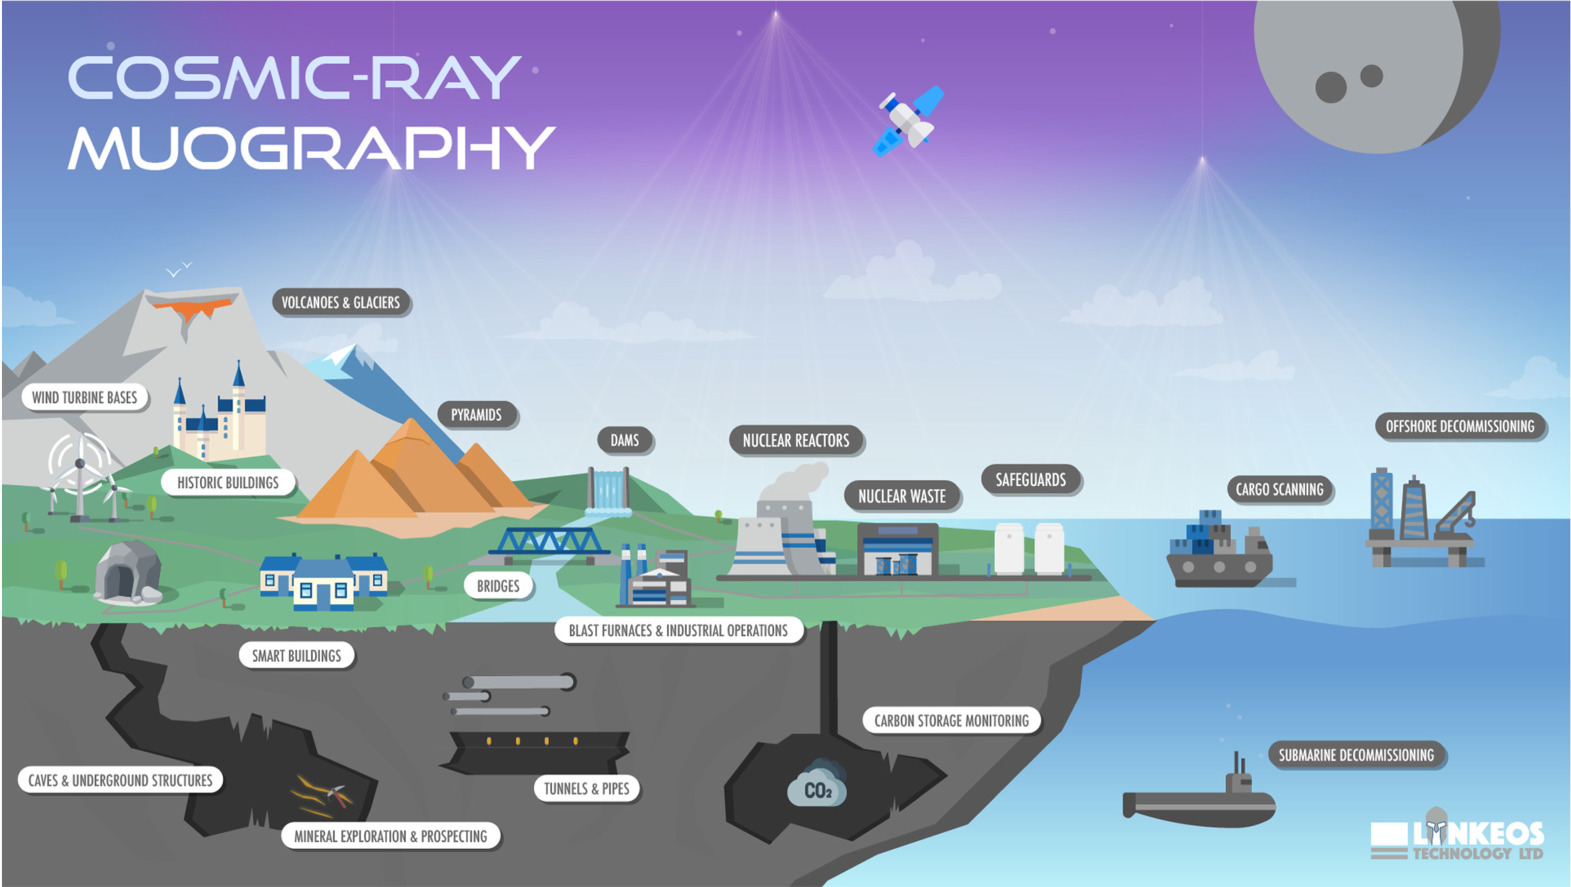
\includegraphics[width=0.5\textwidth]{images/myo_overview.jpg}}
\raggedleft{\footnotesize{\href{https://royalsocietypublishing.org/cms/asset/44e34f40-6c86-4e4a-b3c1-c0c916a6a931/rsta20180049f03.gif}{Muography: overview and future directions Ralf Kaiser}}}

% to see the notes
\setbeameroption{show notes}


\begin{document}

% \maketitle


% \begin{frame}{Hinweise}
  Zu diesem Theme
  \begin{itemize}
    \item Zur Installation des Themese muss mindestens die Datei \texttt{beamerthemetudo.sty} und der Ordner \texttt{logos} in einen Ordner verschoben werden, in dem \LaTeX nach Paketen sucht.
      Dies können sein
      \begin{itemize}
        \item \texttt{TEXMFHOME/tex/latex/tudobeamertheme}. Den Wert von \texttt{TEXMFHOME} bekommen sie über \texttt{kpsewhich --var-value TEXMFHOME}, üblicherweise ist dies \texttt{\$HOME/texmf}.
        \item Der gleiche Ordner in dem Sie ihr Dokument kompilieren
        \item Ein beliebiger Ordner, der in der Variablen \texttt{TEXINPUTS} enthalten ist.
      \end{itemize}
  \end{itemize}
  
  Oneliner zur Installation:\\
  \texttt{\footnotesize\$ cd `kpsewhich --var-value TEXMFHOME` \&\& git clone https://github.com/maxnoe/tudobeamertheme}

  \medskip
  Allgemein zu Beamer und Latex:
  \begin{itemize}
    \item Umfangreicher \LaTeX-Kurs von PeP et Al. \\
      \url{http://toolbox.pep-dortmund.org/notes}
    \item Latex-Beamer Dokumetation:\\
    \url{http://www.ctan.org/pkg/beamer}
  \end{itemize}
\end{frame}

\begin{frame}{Einführung}
  \tableofcontents
\end{frame}

\section{Fonts}
\begin{frame}
  Der Font der im Corporate Design der TU Dortmund vorgesehen ist,
  ist \enquote{Akkurat Office}.

  Falls dieser nicht verfügbar ist, wird als Alternative \enquote{Fira Sans}
  verwendet.

  Für Mathematik wird bei Verwendung von \texttt{xelatex} oder \texttt{lualatex} der Font \enquote{Fira Math} verwendet.
\end{frame}

\begin{frame}{Mathe}
  \begin{align*}
    \nabla \cdot \symbf{B} &= 0 &
    \nabla \cdot \symbf{E} &= \frac{ρ}{ε_0} \\
    \nabla \times \symbf{E} &= -\partial_t \symbf{B} &
    \nabla \times \symbf{B} &= μ_0 \symbf{j} + μ_0 ε_0 \partial_t \symbf{E} &
  \end{align*}
\end{frame}
% \begin{frame}{Agenda}
	\begin{columns}[T]
		\begin{column}{.4\textwidth}
% 			\begin{block}{Your textblock}
				\begin{itemize}
				    \item Motivation: \emph{Landunter} im Stollen!
				    \begin{itemize}
							\item[\to] Das Erbe des Bergbaus
					\end{itemize}
				    \item Lösung: Myonen als "Röntgenstrahlung"
				    \begin{itemize}
				            \item Das Prinzip der Myographie
							\item[\to] Pyramiden, Vulkane und Bergbau 
					\end{itemize}
					\item Myographie im Ruhrgebiet
				    \begin{itemize}
							\item Wie lässt sich ein Wasserpegel untertage messen?
				    		\item Detektor-Zählraten simulieren
				    		\item Ein Bodenprofil im Ruhrgebiet
					\end{itemize}
					
				\end{itemize}
% 			\end{block}
		\end{column}
		\begin{column}{.5\textwidth}
% 			\begin{block}{Your image}
                %% allgemeines cooles myographie bild
				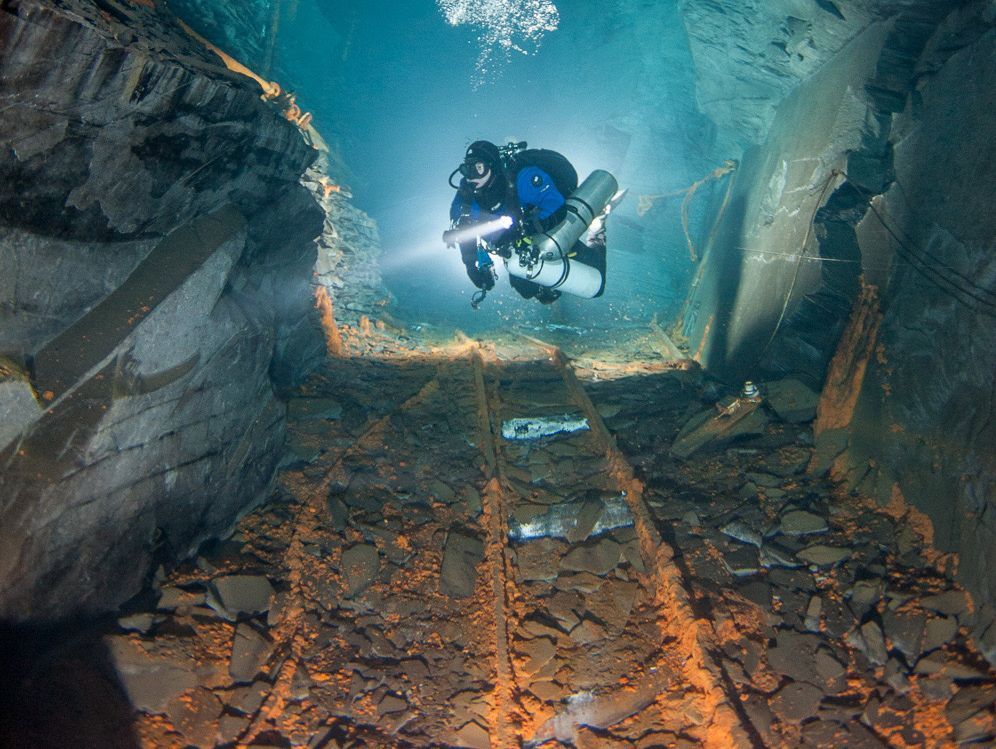
\includegraphics[width=\textwidth]{images/wasser_stollen.jpg}
				\raggedleft{\footnotesize{\href{https://www.spiegel.de/reise/deutschland/bergwerk-nuttlar-in-bestwig-tauchen-mit-tunnelblick-a-914935.html}{[Spiegel - uwpics-bjoern.de]}}}
% 			\end{block}
		\end{column}
	\end{columns}
\end{frame}
\begin{frame}{TITEL}
	\begin{columns}[T]
		\begin{column}{.45\textwidth}
			%\begin{block}{Your textblock}
				\begin{itemize}
					\item HAUPTPUNKT
						\begin{itemize}
							\item[\to] UNTERPUNKT
						\end{itemize}
				\end{itemize}
			%\end{block}
		\end{column}
		\begin{column}{.55\textwidth}
			%\begin{block}{Your image}
				
\includegraphics[width=\textwidth]{images/e5-logo.png}
			%\end{block}
		\end{column}
	\end{columns}
	\note[item]{Verschiedene Botenteilchen von Quelle}
	\note[item]{Neutrinos Nachteil: nur schwache WW $\to$ schwierige Detektion}
\end{frame}



%\nocite{*}
%\printbibliography

\end{document}
